\setchapterstyle{kao}
\setchapterpreamble[u]{\margintoc}
\chapter{RoboModule Motor Driver}
\labch{34RMD}

\section{Function Description}
The RoboModule Motor Driver is used for the controlling of Rope-Climbing Robot climbing motor, it should be 
used with Can Analysis \ref{ch:51CA}. 
% \sidenote{  \href{https://www.akm.com/cn/zh-cn/technology/technical-tutorial/basic-knowledge-magnetic-sensor/hall-sensors/}
% {Introduction of Hall sensors link} }. 
% \begin{figure}[hb]
% 	\includegraphics[width=0.45\textwidth]{4101_motor1.jpg}
% 	\caption[Mona Lisa, again]{It's Mona Lisa again.}
% 	\labfig{fig411_cleaningMotor}
% \end{figure}

Application: large current BLDC, replace epos, elmo and minglang; RoboMasters.

\begin{figure}[htb]	
	\centering
	\begin{subfigure}
		\centering
		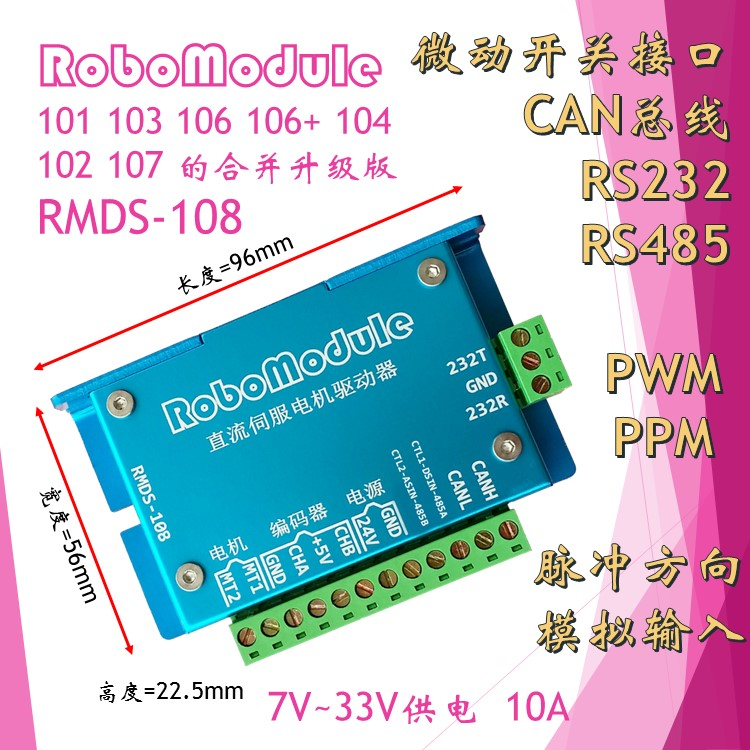
\includegraphics[width=2in]{3401_motordriver.jpg}
		% \caption{motor with reduction detail}\label{fig:4101}		
	\end{subfigure}
	\quad
	\begin{subfigure}
		\centering
		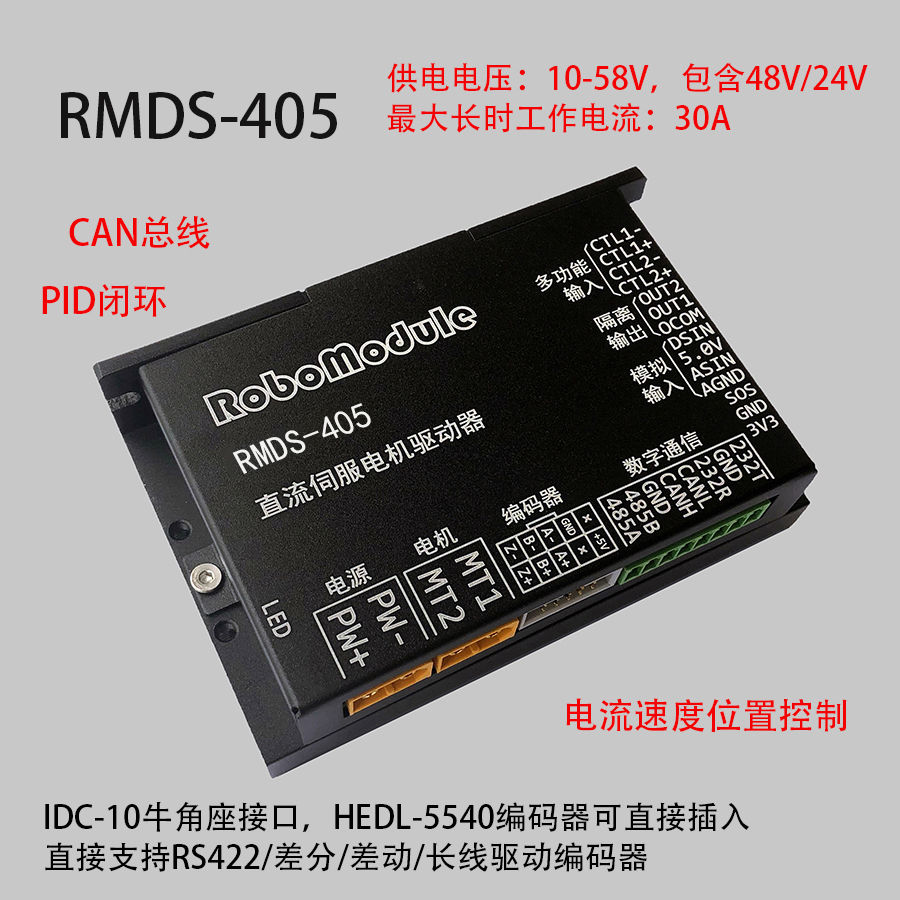
\includegraphics[width=2in]{3402_motordriver.jpg}
		% \caption{motor with brand}\label{fig:4102}
	\end{subfigure}
	% \begin{subfigure}
	% 	\centering
	% 	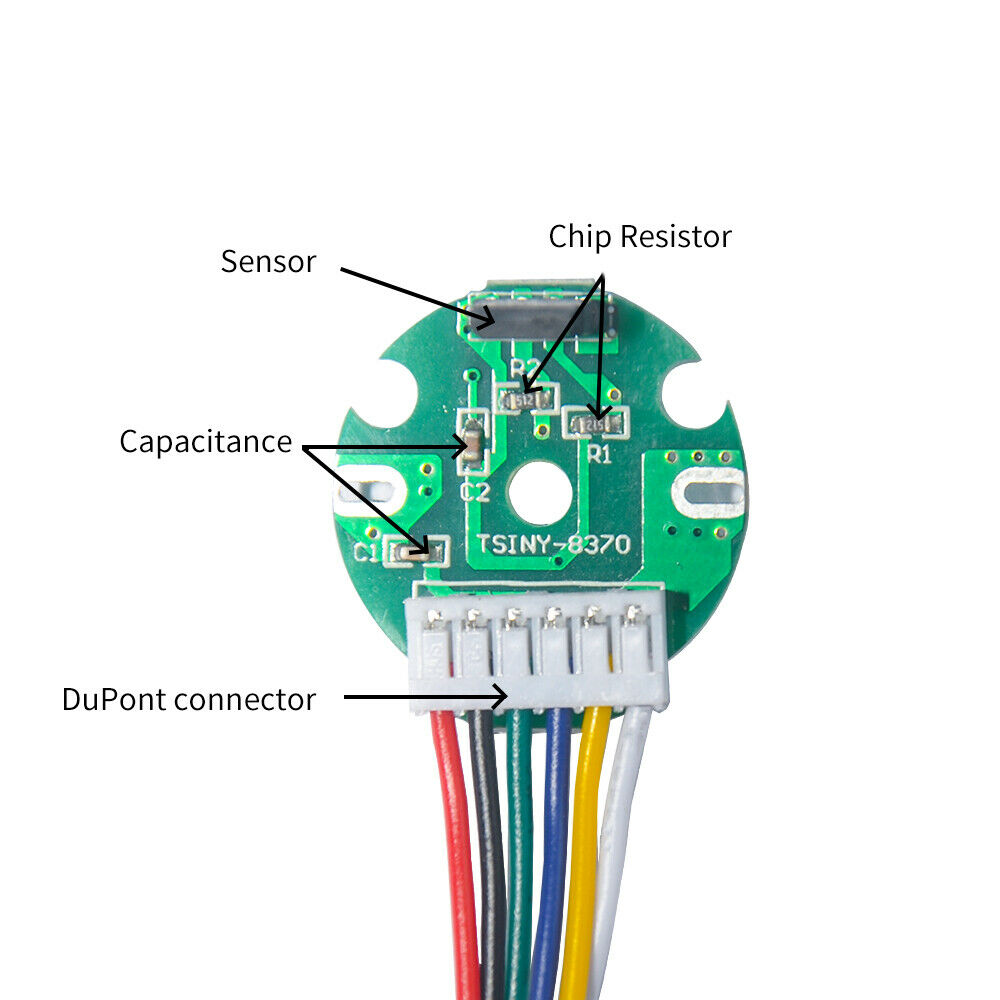
\includegraphics[width=2in]{412_hallencoder.jpg}
	% 	% \caption{motor with brand}\label{fig:4102}
	% \end{subfigure}
	\caption[RoboModule Motor Driver]{ 
		RoboModule Motor Driver		
			}\label{fig:340}
\end{figure}
% \marginnote[-12pt]{
	
% 	}
\section{Purchase Info}
Purchase:
\begin{enumerate}
	\item brand: RoboModule
	\item type: RMDS-403 and RMDS-109
	\item link: \href{https://item.taobao.com/item.htm?id=43995228864}{taobao link} 
	\item price: 700RMB and 370RMB
	\item data: June. 2020
	\item RP: SGL, clear
\end{enumerate}

Supporting Material:
\begin{enumerate}
	\item RoboModule website: \url{http://www.robomodule.net/download.html}
    \item Always refer to: online instructions of 003(common problems) and 011 (can protocol), 
      They have been downloaded in ros package robomodule sheet folder on {\color{red} September 19, 2020.}.
	\item telephone: +86-18503054370
    \item rs232 serial wire purchase link: \url{https://detail.tmall.com/item.htm?id=39113690170 }
\end{enumerate}


\section{Instruction for Connection}
\begin{marginfigure}[-2cm]
	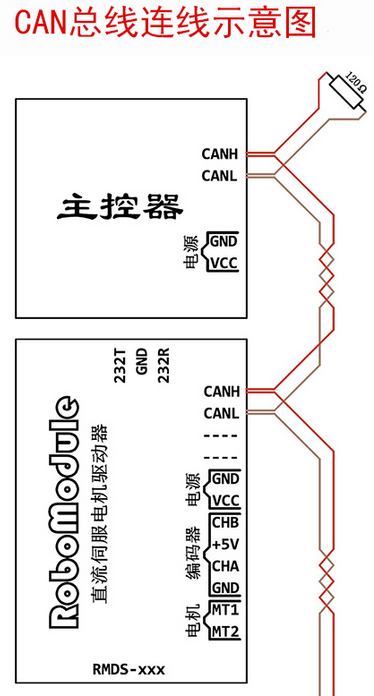
\includegraphics[width=0.8\textwidth]{3434_RMDS_cn_can2controller.png}
	\caption[arduino ttl to can ]{arduino ttl to can }
	\labfig{fig3434:can2controller}
\end{marginfigure}
\subsection{Windows}

In windows,  followings should be done:
\begin{enumerate}
	\item set feedback part (encoder) parameters, write in encoder resolution.
	\item adjust motor and encoder direction, using GUI velocity mode, check pop data and pwm set data direction, if not same, change direction of the Motor.
    \item check the using mode in the GUI, velocity and velocity-position mode are using in our program.
    \item set the driver's group and id number. here {\color{red}403: G0, id1; 109: G1, id1}.
\end{enumerate}
\begin{marginfigure}
	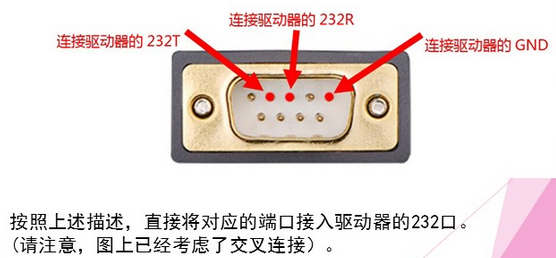
\includegraphics[width=1\textwidth]{3432_RMDS_cn_232pins.png}
	\caption[RS232 Pins]{RS232 Pins connection: {\color{red} 2:232T; 3:232R; 5:GND.} }
	\labfig{fig3432:232pins}
\end{marginfigure}

\begin{marginfigure}
	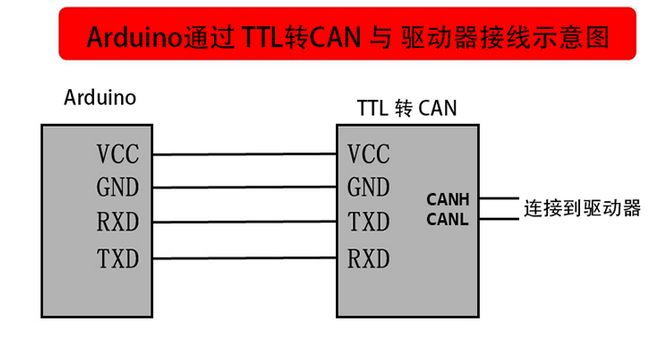
\includegraphics[width=1\textwidth]{3433_RMDS_cn_arduino_ttl_can.png}
	\caption[arduino ttl to can ]{arduino ttl to can }
	\labfig{fig3433:ttltocan}
\end{marginfigure}

communication rate:
\begin{enumerate}
	\item can: 1000khz
	\item 232: 115200
	\item 485: 115200
\end{enumerate}

\begin{figure}[htb]
	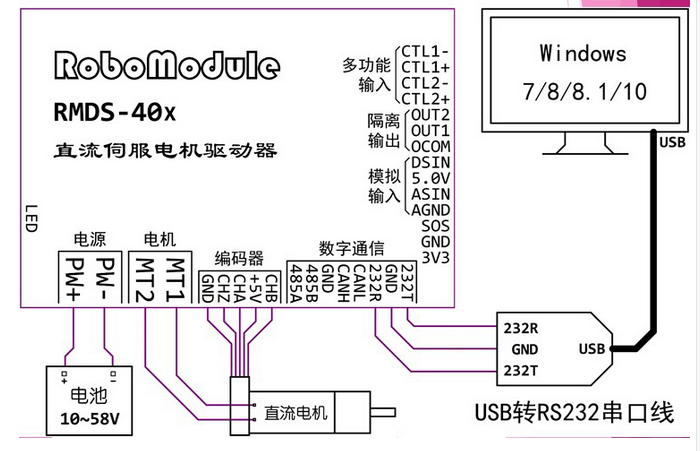
\includegraphics[width=1\textwidth]{3431_RMDS_cn_windows_tune.png}
	\caption[tune wire connection]{ 
		tune wire connection.		 
		}
	\labfig{fig3431:windows_tune}
\end{figure}
% 1234

% wire definition in encoders:
% \begin{enumerate}
% 	\item {\colorbox{red}W red}: M1, motor + positive
% 	\item {\colorbox{black}W black}: GND, encoder power supply - negative
% 	\item {\colorbox{yellow}W yellow}: C1, encoder signal A phase
% 	\item {\colorbox{green}W green}: C2, encoder signal B phase
% 	\item {\colorbox{blue}W blue}: 3.3/5v, encoder power supply + positive
% 	\item {\colorbox{white}W white}: M2, motor - negative 
% \end{enumerate}

\section{Mechanical Specification}
It includes magnetic motor main part, reduction,  D shaft and a magnetic incremental encoder.

Motor specification:
\begin{enumerate}
	\item RMDS109:  W: 56mm, L: 96mm; H: 22.5mm
	\item RMDS403: W: 76mm, L: 118mm; H: 33mm
\end{enumerate}

\begin{figure}[htb]
	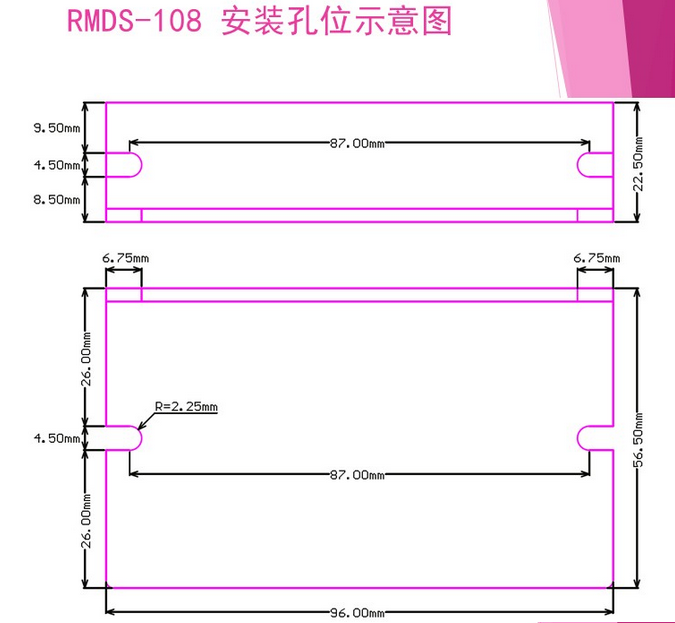
\includegraphics[width=0.8\textwidth]{3441_RMDS_109_mech_install.png}
	\caption[RMDS109 mechanical installation]{ 
		RMDS109 mechanical installation. (109 is same as 108), in 403,401, just care 87mm to 105mm		 
		}
	\labfig{fig3441_mech_install}
\end{figure}

\section{Electrical Specification}
RMDS specification:
\begin{marginfigure}[-3cm]
	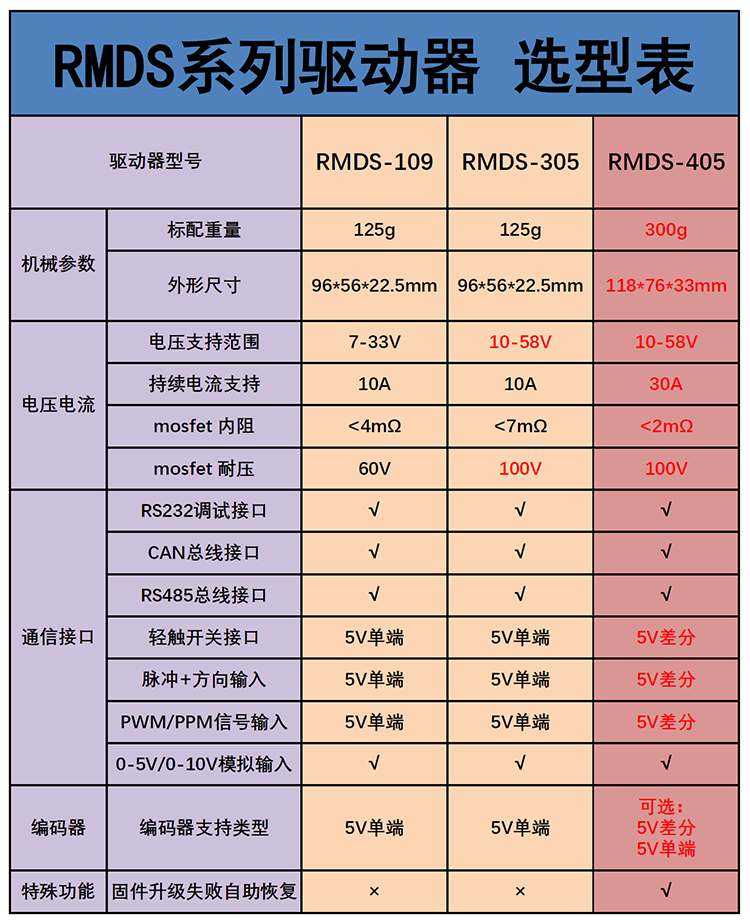
\includegraphics[width=1\textwidth]{343_RMDS_el_sp.png}
	\caption[RMDS Driver electrical specification]{ 
		RMDS Driver electrical specification, here we have used the formal version of them, 403 and 109.		 
		}
	\labfig{fig:343}
\end{marginfigure}
RMDS109:
\begin{enumerate}
	\item power supply: 7 \textasciitilde 33v
	\item constant output current: 10A
	\item max speed: -32768 \textasciitilde +32767 RPM
\end{enumerate}

RMDS403:
\begin{enumerate}
	\item power supply: 10 \textasciitilde 58v
	\item constant output current: 30A
	\item max speed: -32768 \textasciitilde +32767 RPM
\end{enumerate}


\section{others}
\subsection{how to use 12v motor in 24v power supply }
set in the windows GUI, set PWM and current limitation.
\begin{figure}[!htb]
	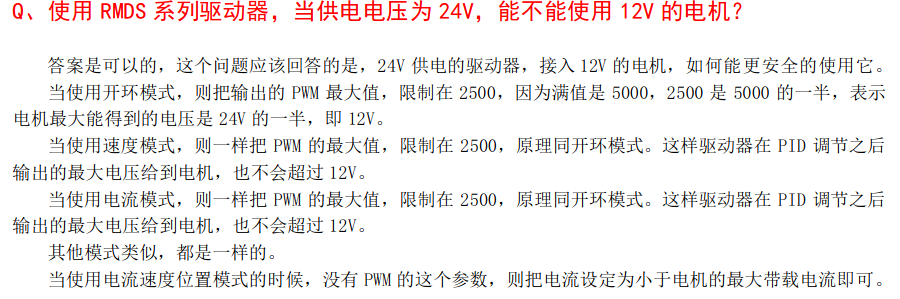
\includegraphics[width=0.8\textwidth]{345_use24vfor12vmotor.png}
	\caption[how to use 12v motor in 24v power supply]{ 
		how to use 12v motor in 24v power supply.		 
		}
	\labfig{fig:345}
\end{figure}

\subsection{how to judge differential encoder and single port encoder }
two AB or single AB
\begin{figure}[!htb]
	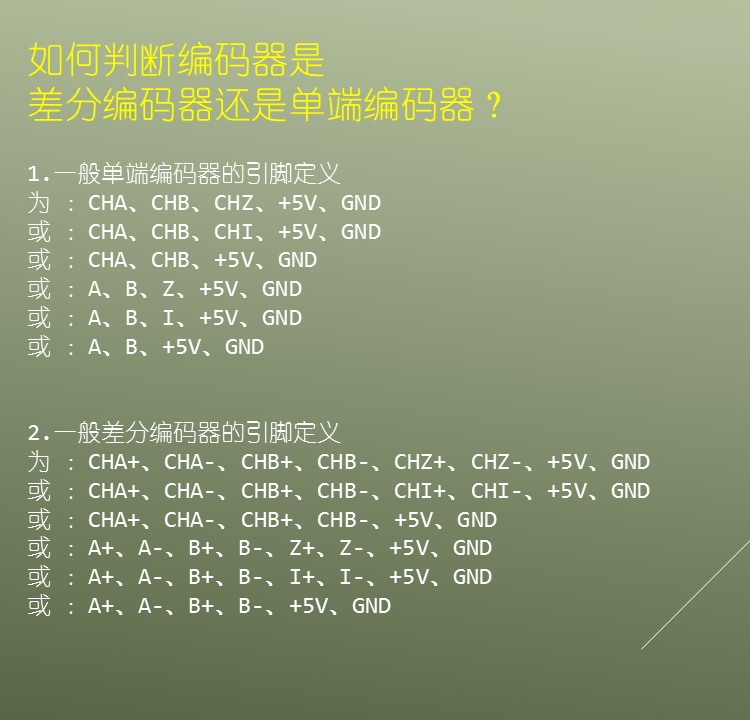
\includegraphics[width=0.5\textwidth]{344_diff_encoder_judge.png}
	\caption[how to judge differential encoder and single port encoder]{ 
		how to judge differential encoder and single port encoder.		 
		}
	\labfig{fig:344}
\end{figure}

\section{Protocol}
mode value:
\begin{table}[htb!]
	\caption[RoboModule mode value]{RoboModule mode value table.}
	\labtab{341_rmv}
	\begin{tabular}{ c c }
		\toprule
		mode name & DATA[0] in init cmd \\
		\midrule
		open loop  & 0x01  \\
		\midrule
		current  & 0x02  \\
		\midrule
		velocity  & 0x03  \\
		\midrule
		position  & 0x04  \\
		\midrule
		vel-position  & 0x05 \\
		\midrule
		current-vel  & 0x06  \\
		\midrule
		current-position  & 0x07  \\
		\midrule
		current-vel-pos  & 0x08  \\
		\bottomrule
	\end{tabular}
\end{table}

command index for each mode is the value of mode value + 1;